\section{Phase d'initialisation}
\subsection{Peuplements}
Dans la fenêtre \textit{Wiewertabs}, cliquer sur l'icône \textit{Edit civilisation}, sur la droite la liste des peuplements existants (par défaut  rattaché à l'environnement par défaut).
Pour créer un nouveau peuplement, cliquer sur l'icône \textit{create new civilization},   donner son nom (par exemple Volque), sa population (par exemple 100) et valider (touche entrée).

\subsection{Environnement physique}

Dans la fenêtre \textit{Wiewertabs}, cliquer sur l'icône \textit{Edit environnement}, la liste des terrains attribuables aux \textit{patches} et  définis dans le dossier de la simulation apparait dans la partie droite de la fenêtre (cf. Figure \ref{ENV}).
\begin{figure}[!ht]
	\begin{center}
	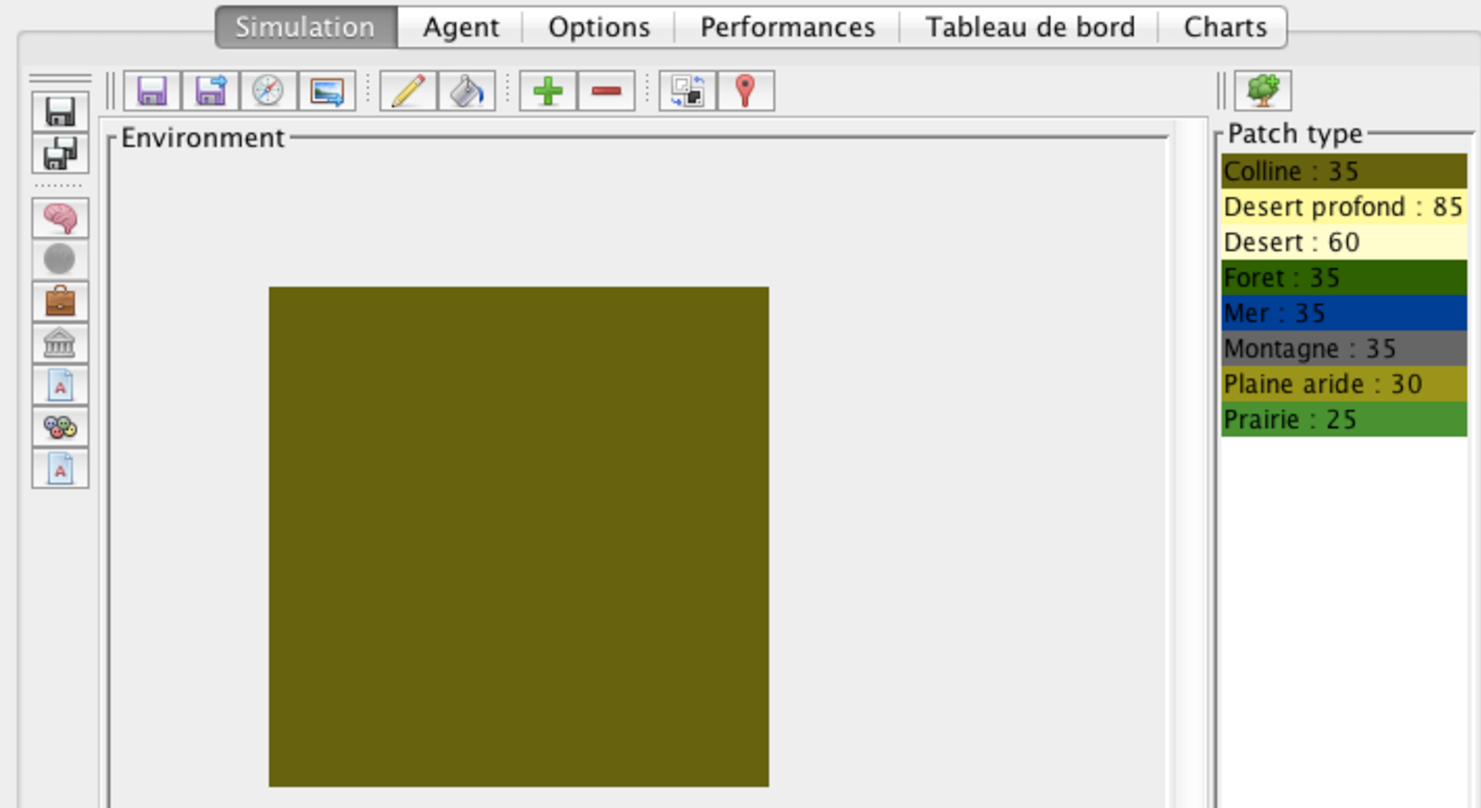
\includegraphics[scale=0.4]{DocumentationSimulation/Env.pdf}
	\caption[ENV]{Environnement \\}
	\label{ENV}
	\end{center}
	\end{figure}
	
Pour la simulation deux terrains sont utilisés \textit{Forêt} et \textit{Prairie} avec une valeur liée à leur facilité de traversée (\textit{passability}).

Les modifications sur un terrain se font par l'intermédiaire d'un clic droit sur le terrain voulu.
On peut alors éditer, changer la couleur ou supprimer le terrain.
Si on édite notre exemple (cf. Figure \ref{Ter} ), on observe le terrain \textit{Prairie} avec la valeur 25 pour \textit{passability}, puis une liste d'attributs correspondant chacun à un type de ressource disponible sur le terrain. Pour chaque ressource on peut attribuer une valeur initiale et une valeur de croissance (à chaque\textit{ tick}). 

\begin{figure}[!ht]
	\begin{center}
	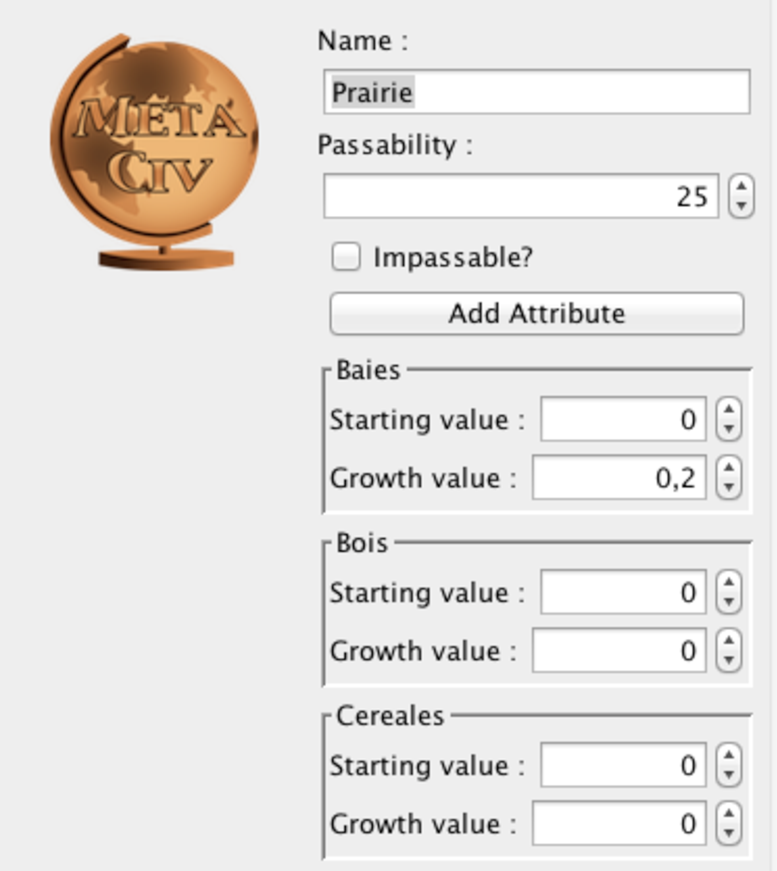
\includegraphics[scale=0.5]{DocumentationSimulation/terrain.pdf}
	\caption[Ter]{Edition d'un terrain \\}
	\label{Ter}
	\end{center}
	\end{figure}


% On peut aussi ajouter de nouveaux attributs (ressources).

Dans la partie centrale de la fenêtre, l'environnement global peut être construit, dimensions (icône boussole \textit{set environment bounds}), chargement d'un environnement existant (icône \textit{Load Environment}), définir à partir d'une image (\textit{generate an environment from an existing picture}) ou dessiner (icône crayon et pot de peinture). 

On peut sauvegarder l'environnement (icône disquette), choisir l'environnement de la simulation (qui peut donc être un autre) icône \textit{choose environment to use for simulation}, et ajouter des ressources à l'environnement (icône \textit{manage pheronom}).


Dernière chose, situer le ou les peuplements sur l'environnement : pour cela clic droit sur la position voulue (possibilité de zoom) et donner le nom du peuplement dans la fenêtre qui s'ouvre (et penser à sauvegarder).

\begin{figure}[!ht]
	\begin{center}
	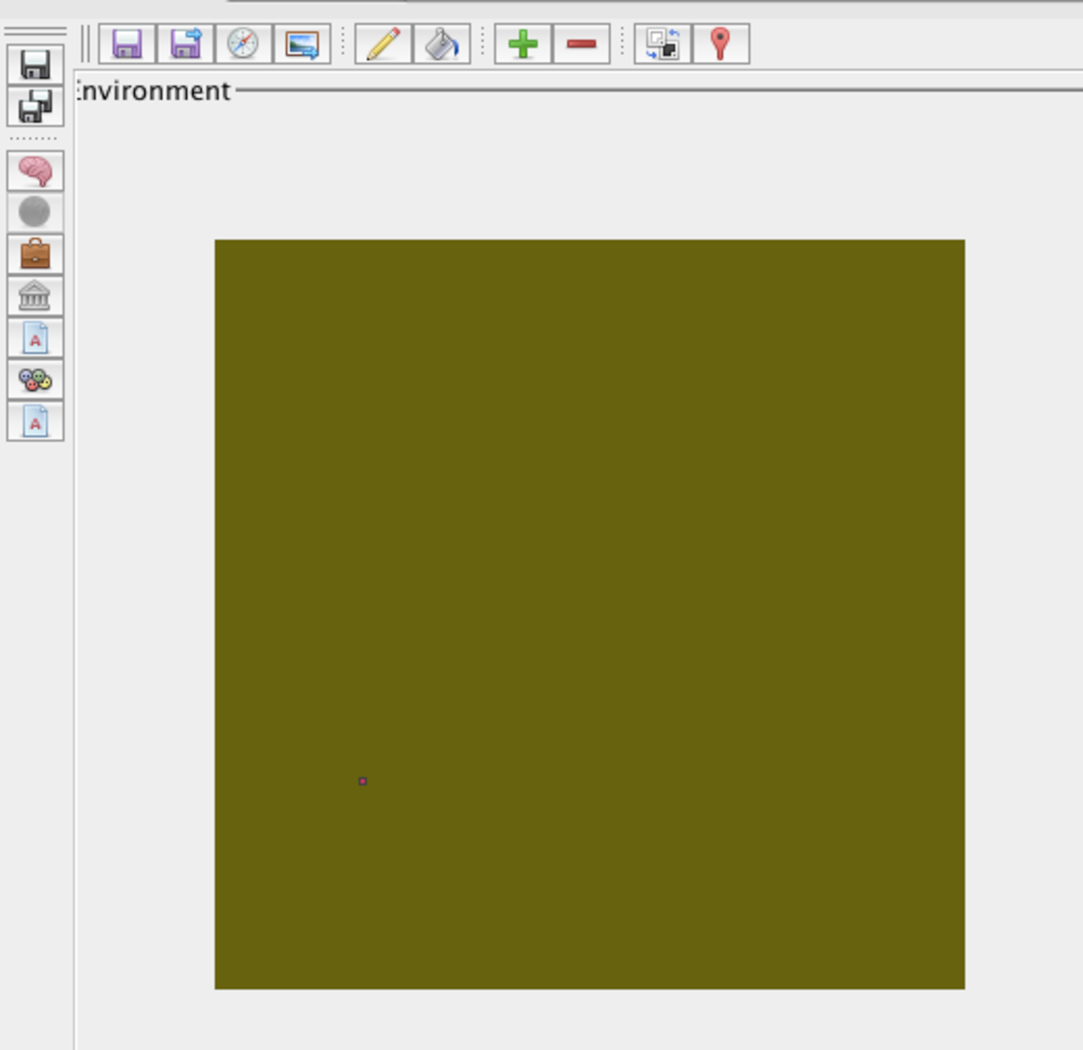
\includegraphics[scale=0.4]{DocumentationSimulation/Local.pdf}
	\caption[Lo]{Localisation du peuplement, le point marque la localisation}
	\label{Lo}
	\end{center}
	\end{figure}
	
\subsection{Les objets}
Dans la fenêtre \textit{Wiewertabs}, cliquer sur l'icône \textit{Edit Item}.

Sur la partie droite une liste d'objets apparaît et en cliquant sur l'icône \textit{Add Item} on accède à la fenêtre suivante (cf. Figure \ref{Obj}).

\begin{figure}[!ht]
	\begin{center}
	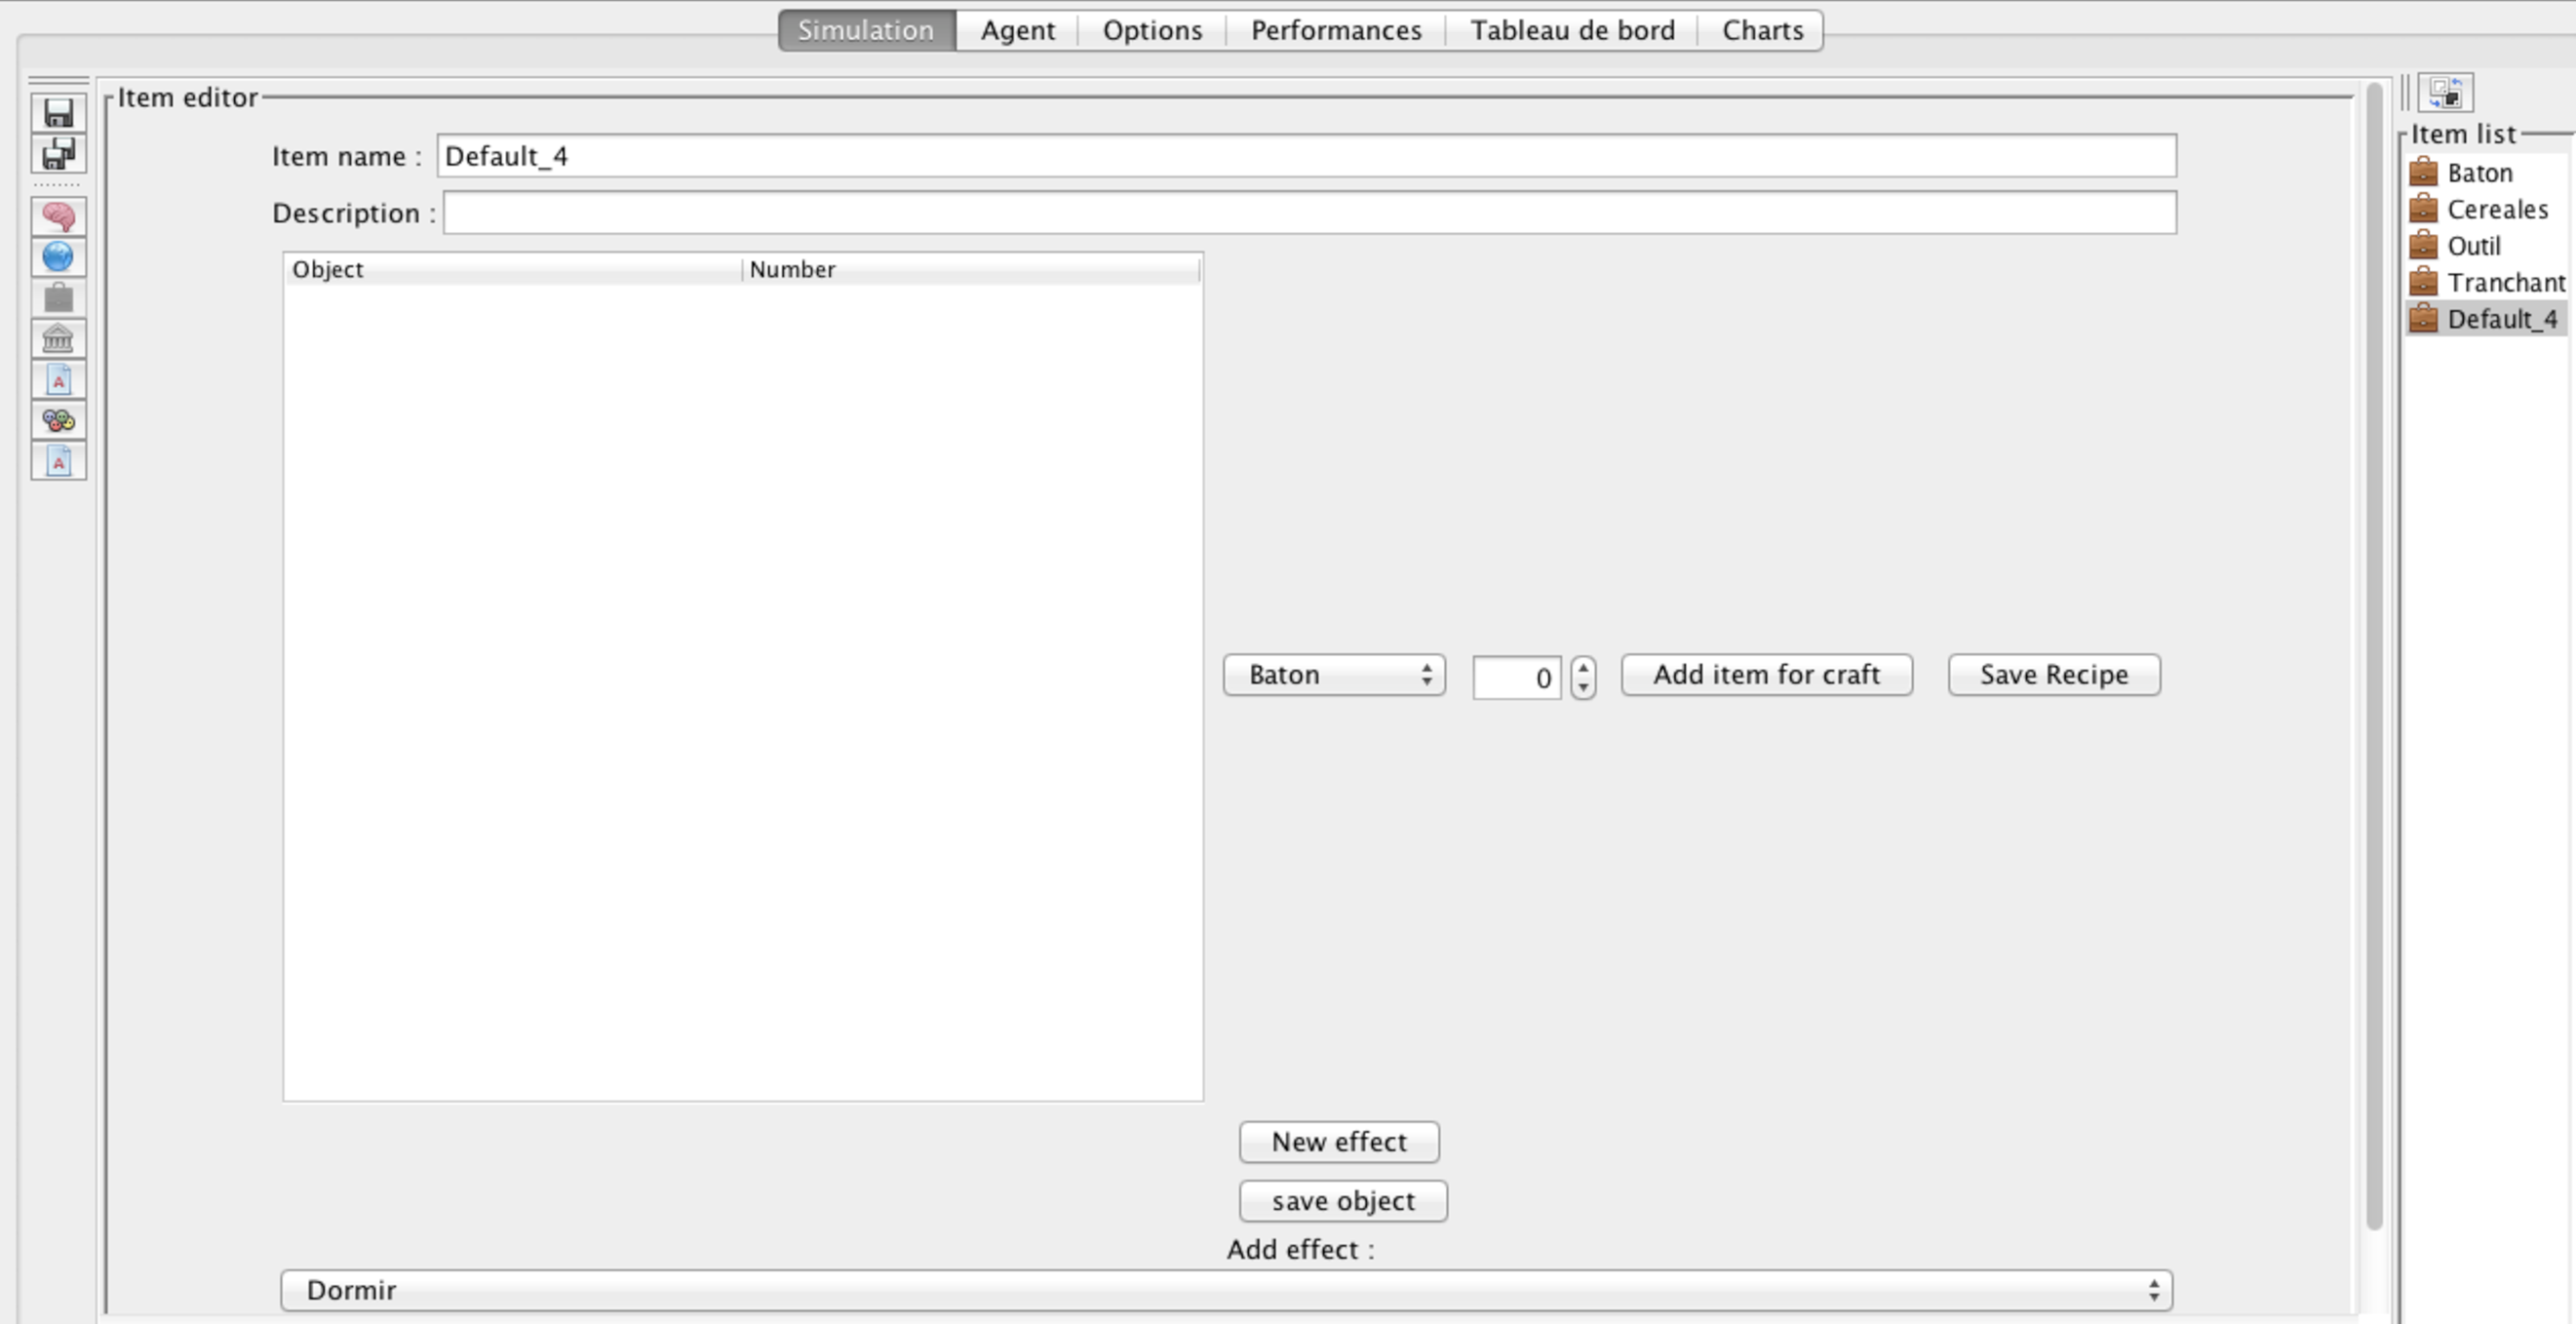
\includegraphics[scale=0.3]{DocumentationSimulation/Objet.pdf}
	\caption[Obj]{Ajout d'objet \\}
	\label{Obj}
	\end{center}
	\end{figure}
	
Dans cette fenêtre donner un nom et une description à l'objet avant de sauvegarder.

Si l'on souhaite créer des descriptions d'objet complexe, on peut saisir le nom et le nombre d'éléments constitutifs (ce qui constitue la recette ou \textit{recipe}). 

On peut de plus ajouter des effets existants ou en créer de nouveaux (cf. Figure \ref{Ob2}).
\begin{figure}[!ht]
	\begin{center}
	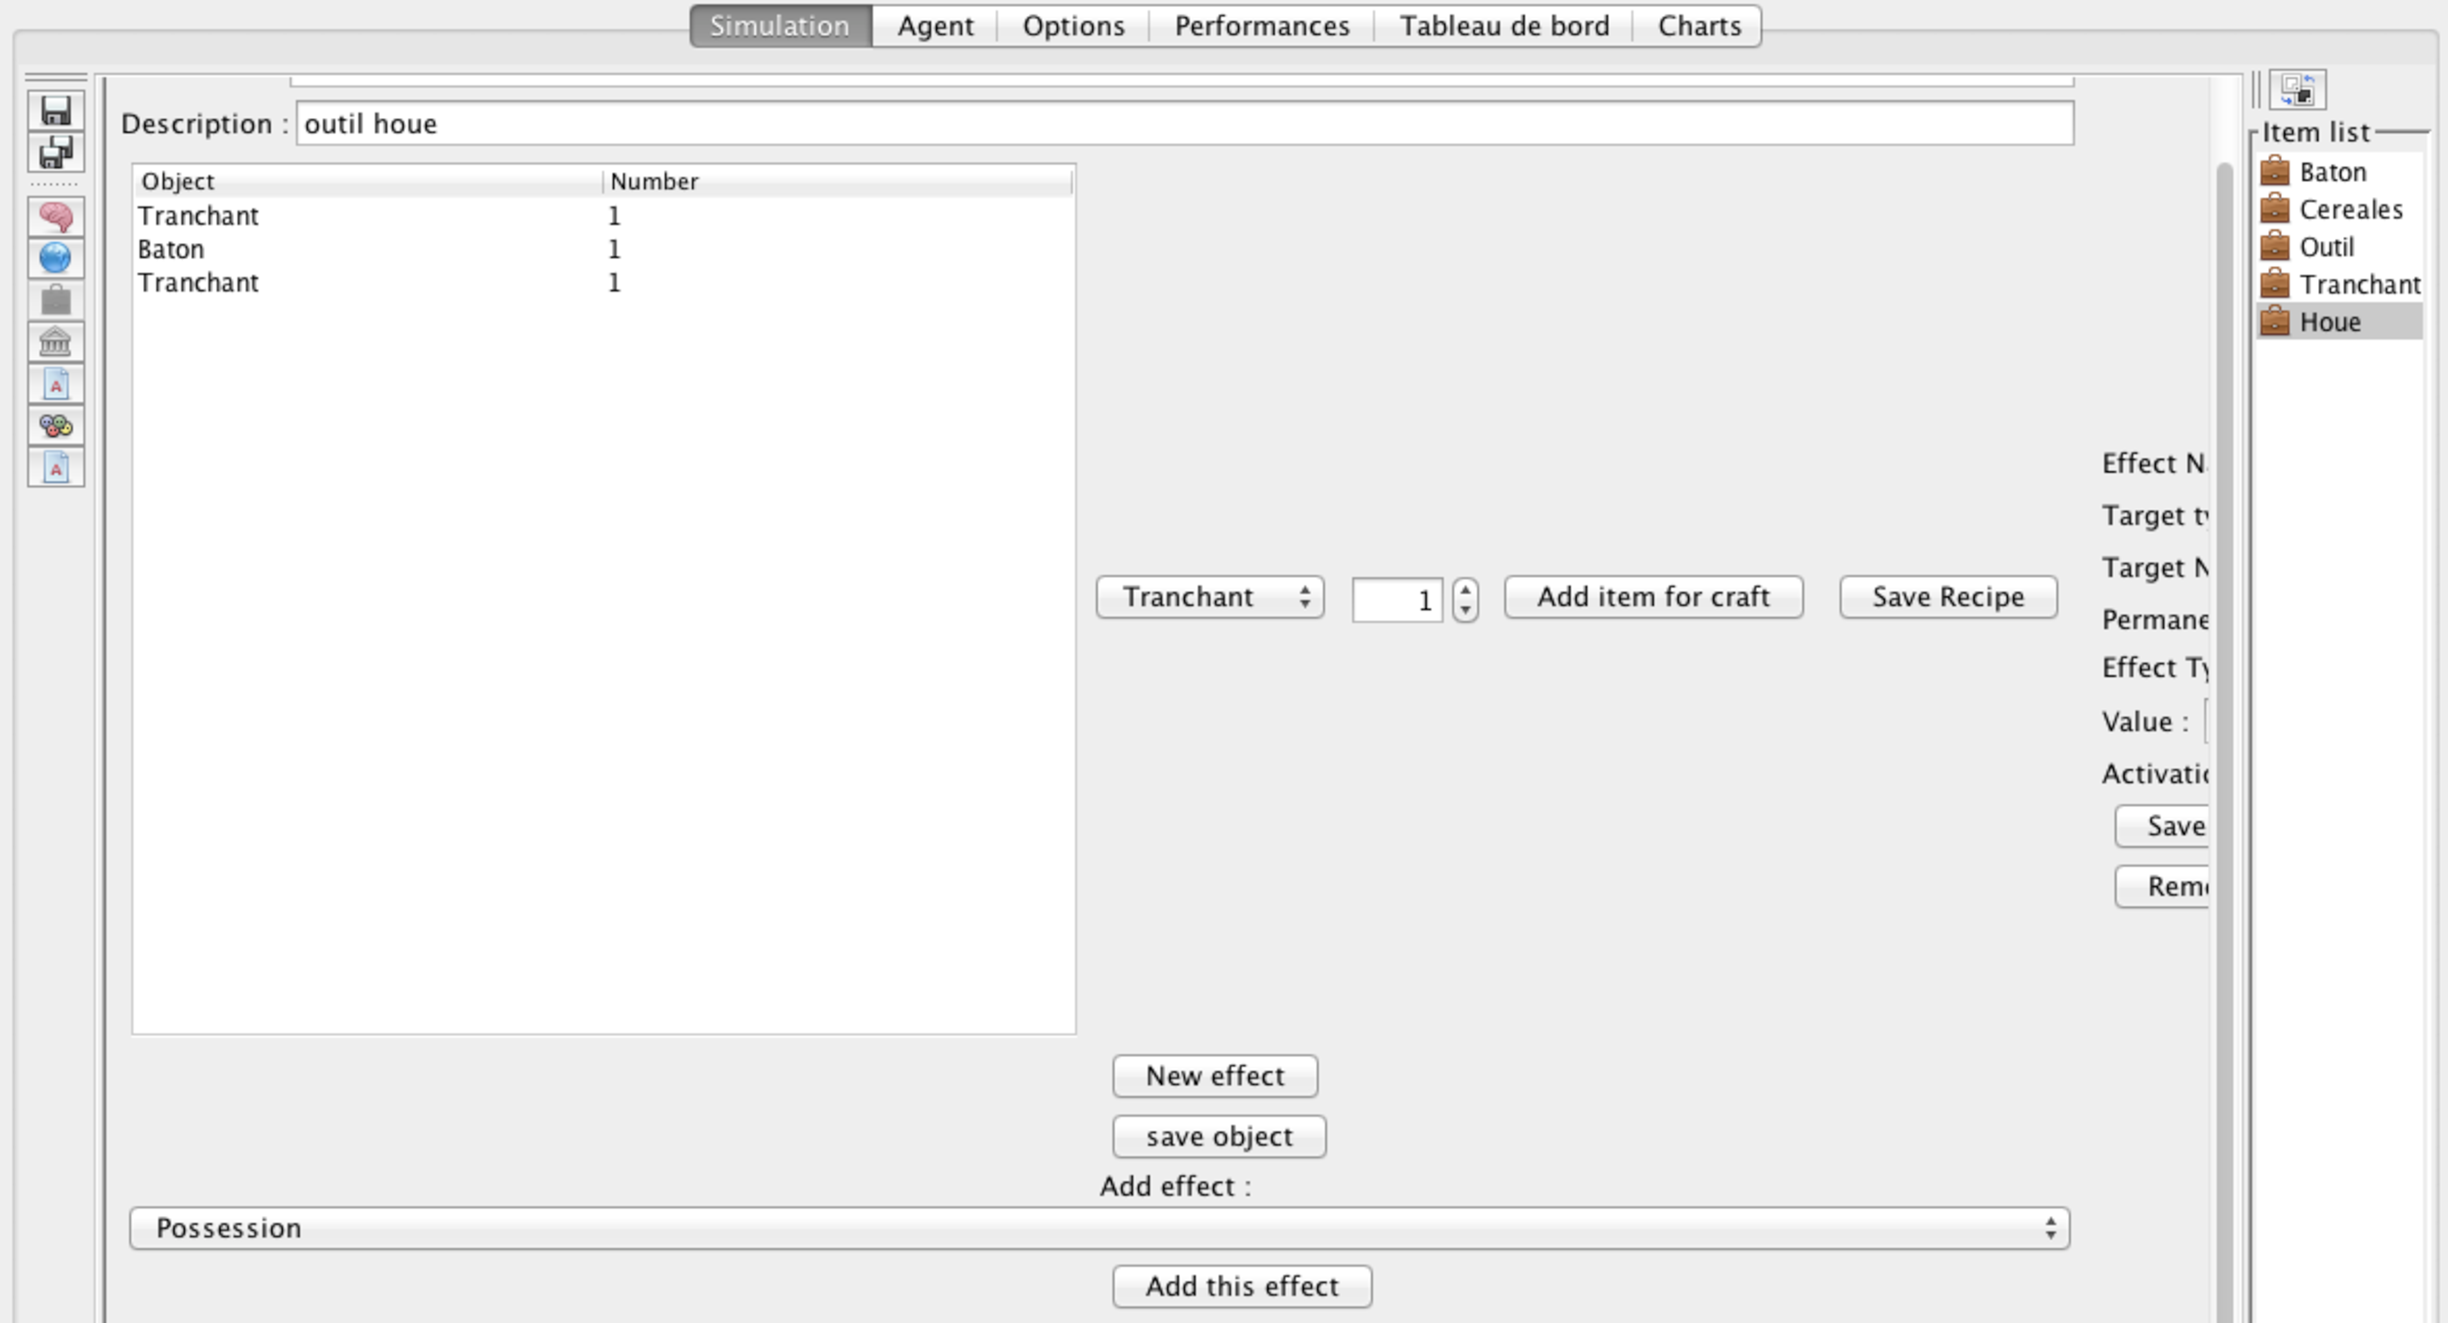
\includegraphics[scale=0.3]{DocumentationSimulation/Objet2.pdf}
	\caption[Ob2]{Objet complexe \\}
	\label{Ob2}
	\end{center}
	\end{figure}
	
En ce qui concerne les effets (cf. Figure \ref{EF2}), tout effet a un nom, une cible qui peut être un attribut (caractéristique de l'agent) ou un cogniton % action. 
Le type de cible étant choisi, on détermine la cible exacte, la durée de l'effet (permanent ou non c'est-à-dire  lié à la durée de vie de l'objet), ce qu'il fait (\textit{set, add, remove}) sur la cible en terme de valuation et en fonction de toute action relative à la création, à l'utilisation et à la destruction de l'objet auquel l'effet est rattaché.

\begin{figure}[!ht]
	\begin{center}
	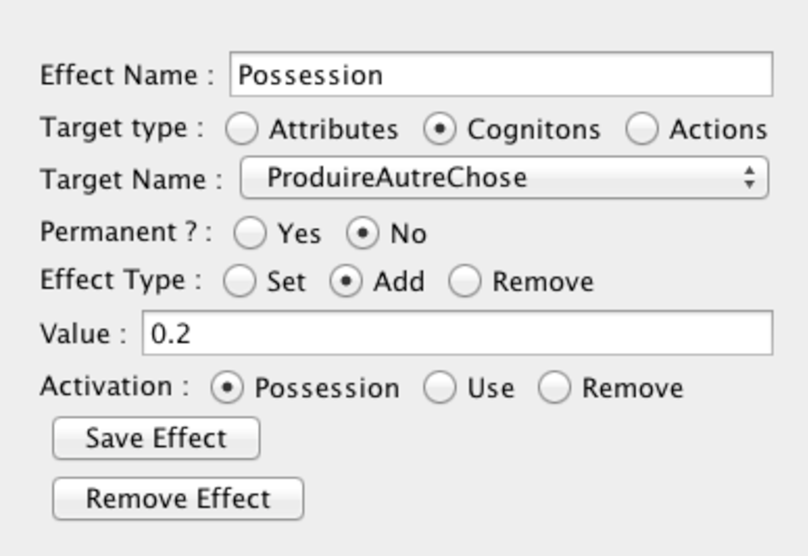
\includegraphics[scale=0.6]{DocumentationSimulation/effet.pdf}
	\caption[EF2]{Effet pour un objet \\}
	\label{EF2}
	\end{center}
	\end{figure}
	
	Exemple, l'objet \textit{Houe} a pour effet \textit{Possession} dont la cible est le cognition \textit{Produireautrechose}, cet effet est transitoire (appliqué tant que l'agent possède la houe), son action sur le cognition est \textit{add} (ajouter) la valeur 0.2 au poids de celui-ci, son activation sera effective chaque fois qu'un agent ajoutera une \textit{Houe} à son inventaire.

\newpage
	
	
\subsection{Les aménagements ou infrastructures}	
		Dans la fenêtre \textit{Wiewertabs}, clicquer sur l'icône \textit{Edit amenagement}, sur la droite on dispose de la liste des aménagements existants.
Pour créer un nouvel aménagement, cliquer sur l'icône \textit{create new amenagement}, donner son nom (par exemple Champ) et sauvegarder.

\begin{figure}[!h]
	\begin{center}
	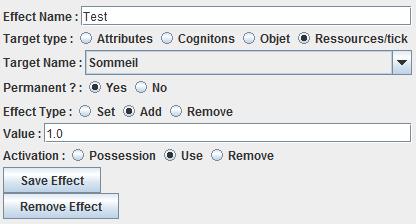
\includegraphics[scale=0.6]{DocumentationSimulation/images/effetsA.png}
	\caption[EFA]{Effet pour un aménagement \\}
	\label{EFA}
	\end{center}
	\end{figure}

 Tout comme pour les objets,  il est possible de saisir une recette pour la conception d'aménagements complexes, le processus étant identique à celui présenté dans la section sur les objets.
 De même, les aménagements peuvent avoir des effets ceux ci étant un peu différents de ceux présentés pour les objets (cf. Figure \ref{EFA})
 
 En effet,  les aménagements  ont la possibilité d'avoir pour cible (en sus des attributs ou caractéristiques d'agent et des cognitions)  des objets ou des ressources, et dans ce cas, l'effet ajoutera, modifiera ou bien supprimera l'objet sélectionné de l'inventaire, ou bien, modifiera, ajoutera, modifiera ou supprimera la ressource ciblée présente sur le patch où se situe l'aménagement.
	
\section{Phase de modélisation \\ Le canevas : cogniton, plan, action}

	La création d'un nouveau cogniton se fait en cliquant sur l'icône 
\includegraphics{DocumentationSimulation/images/newcogni.png}. 
	
	Un nouveau cogniton est alors créé sous la forme d'une ellipse portant le nom "Nouveau cogniton". 
	
\begin{figure}[!ht]
	\begin{center}
	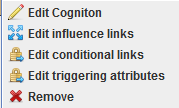
\includegraphics[scale=0.6]{DocumentationSimulation/images/interface.png}
	\caption[Interface]{Interface d'édition de cogniton\\}
	\label{Interface d'édition de cogniton}
	\end{center}
	\end{figure}

Un clic droit sur ce dernier permet d'ouvrir l'interface d'édition (cf. Figure \ref{Interface d'édition de cogniton}). 

Le premier lien permet de donner le nom du cogniton, son type (\textit{ Belief} s'il s'agit d'une croyance de l'agent, même si il s'agit d'une croyance populaire, \textit{Percept} s'il s'agit d'une perception de l'agent, \textit{Skill} s'il s'agit d'une compétence ou d'un savoir-faire, \textit{Trait} s'il s'agit d'une caractéristique psychologique de l'agent et \textit{Culturon} s'il s'agit d'un cogniton partagé par un groupe), et ses pourcentages de chances d'apparition au lancement de la simulation.

Vient ensuite l'édition des \textit{liens d'influence}, à savoir, spécifier quels plans vont être influencés par ce cogniton et dans quelle mesure vont ils l'être. Pour cela, l'on doit sélectionner le plan à influencer ainsi décider le poids de cette influence sur le plan en question. Une fois toutes les influences définies cliquer sur le bouton \textit{OK} pour les enregistrer dans la simulation.

Dans le même menu se trouve l'édition des\textit{ liens conditionnels}. Ces liens spécifient les actions pour lesquelles ce cogniton doit exister obligatoirement dans l'esprit de l'agent pour qu'elle s'exécute. Pour les spécifier il suffit de sélectionner un à un les plans à lier avec l'existence de ce cogniton dans la liste déroulante, puis, cliquer sur le bouton \textit{OK} pour terminer.

Enfin cette interface permet la création de \textit{triggers}. Ces \textit{triggers} permettent de réguler l'apparition d'un cogniton dans l'esprit d'un agent en fonction de la valeur des caractéristiques de ce dernier. Comme un \textit{trigger} est un déclencheur du type \textit{si condition alors}, la création d'un \textit{trigger} se fait en définissant la condition de déclenchement, c'est-à-dire, en sélectionnant la caractéristique de l'agent à comparer, la fonction de comparaison à utiliser, et enfin, la valeur de comparaison. Le cogniton ne se déclenchera, ainsi, dans l'esprit de l'agent, que si cette condition est respectée. 
Il est possible de définir plusieurs conditions au sein d'un même 
 \textit{trigger} . Une fois ces conditions définies, cliquer sur le bouton \textit{OK} pour finir la création du trigger.
 

	
